\documentclass{article}
\usepackage[utf8]{inputenc}
\usepackage[T2A]{fontenc}
\usepackage[russian]{babel}
\usepackage{indentfirst}
\usepackage{graphicx}
\usepackage{amsmath}
\usepackage{amssymb}

\sloppy

\title{Методология разработки решений на основе искусственного интеллекта}
\author{Сосновский Михаил, 341 группа}
\date{}

\begin{document}

\maketitle

\section{Решающие деревья для Феди}

\subsubsection*{Условие}

Никита — электротехник, сын которого, Федя, изучает машинное обучение. Никита придумал конструктор, имитирующий работу решающего дерева для решения задачи бинарной классификации точек на плоскости, где точка описывается признаками $(x_1, x_2)$. Каждой вершине решающего дерева (включая листы) соответствует один элемент конструктора. Конструктор позволяет строить только деревья, решающие правила в вершинах которого имеют вид $[x_i > C]$ для произвольной константы $C$.

Федя позвонил папе и сообщил, что придумал датасет для классификации на 2 класса из 100 различных точек, причём координаты $x_1$, $x_2$ пробегают все возможные значения от 1 до 10. При этом Федя забыл сказать папе, какие точки к какому классу принадлежат. Никите нужно взять на работе достаточное количество элементов конструктора, чтобы Федя смог построить решающее дерево вне зависимости от того, каким классам принадлежат точки. Какое количество элементов ему понадобится?

Иными словами, найдите такое минимальное число $N$, что, вне зависимости от разбиения точек на 2 класса, найдётся решающее дерево, идеально решающее эту задачу классификации, состоящее не более чем из $N$ вершин.

\subsubsection*{Решение}

Раз точки разделены на 2 класса и координаты точек пробегают все возможные значения от 1 до 10, а всего точек 100, то можно представить себе распределение данных точек, как квадратную область размером 10x10 клеток, каждая из которых закрашена одним из двух цветов в зависимости от класса точки.

Таким образом, в худшем случае классы точек будут чередоваться так, что никакие две соседние клетки не будут одного цвета, как на шахматной доске. Тогда, чтобы точно классифицировать каждую точку с помощью дерева решений, потребуется сначала «разрезать» все точки по столбцам (например, с помощью порогов $[x_1 > 1.5]$, $[x_1 > 2.5]$ и т. д.), затем по строкам, а затем посмотреть на каждую точку по отдельности.

Получаем, что в бинарном дереве для разделения 10 столбцов нужно 9 внутренних вершин вида $[x_1 > C]$, т. к. дерево с 10 листьями (различные столбцы) имеет 9 внутренних вершин. Потом каждый столбец необходимо разделить на 10 строк с помощью 9 аналогичных внутренних вершин вида $[x_2 > C]$. Т. к. столбцов всего 10, то получаем $10 \cdot 9 = 90$ внутренних вершин.

Что касается листьев решающего дерева, то в худшем случае их потребуется 100, исходя из того, что при распределением точек в виде шахматной доски любая одноцветная область занимает ровно одну клетку, а таких клеток в квадратной области 10x10 будет 100.

Поскольку полное бинарное дерево с $L$ листьями имеет ровно $2 \cdot L - 1$ вершин, то в данной задаче в худшем случае потребуется не менее $2 \cdot 100 - 1 = 199$ вершин. С другой стороны, 199 вершин достаточно для любого разбиения, потому что можно построить дерево, которое сначала разделяет точки по столбцам (9 вершин), затем в каждом столбцев по строкам (90 вершин) и 100 листьев.

\textbf{Ответ:} Никите нужно взять 199 элементов конструктора, чтобы их гарантированно хватило для любого размеченного Федей набора точек.

\section{Упражнения по корреляции}

\subsection*{Упражнение 4.1}

\subsubsection*{Условие}

Напишите функцию Python, которая на входе принимает два вектора и на выходе выдает два числа: коэффициент корреляции Пирсона и значение косинусного сходства. Напишите исходный код, который следует формулам, представленным в данной главе; не используйте вызовы встроенной в NumPy функции \texttt{np.corrcoef} и встроенной в SciPy функции \texttt{spatial.distance.cosine}. Убедитесь, что два значения на выходе идентичны, когда переменные уже центрированы по среднему значению, и различны, когда переменные не центрированы по среднему значению.

\subsubsection*{Решение}

Напишем функцию, которая на входе принимает два вектора и на выходе выдает два числа: коэффициент корреляции Пирсона и значение косинусного сходства.

\begin{verbatim}
In  [1] import numpy as np

        def get_corr(x, y):
            x = np.array(x, dtype=float)
            y = np.array(y, dtype=float)
            

            cosine = np.sum(x * y) / (
                np.sqrt(np.sum(x ** 2)) * np.sqrt(np.sum(y ** 2))
            )
            
            x -= np.mean(x)
            y -= np.mean(y)
            
            pearson = np.sum(x * y) / (
                np.sqrt(np.sum(x ** 2)) * np.sqrt(np.sum(y ** 2))
            )
            
            return pearson, cosine
\end{verbatim}

Убедимся, что два значения на выходе идентичны, когда переменные уже центрированы по среднему значению.

\begin{verbatim}
In  [2] x1 = np.array([-2, -1, 0, 1, 2])
        y1 = np.array([-4, -2, 0, 2, 4])

        pearson_1, cosine_1 = get_corr(x1, y1)

        print(f"Вектор x: {x1}")
        print(f"Вектор y: {y1}")
        print()
        print(f"Корреляция Пирсона: {pearson_1:.6f}")
        print(f"Косинусное сходство: {cosine_1:.6f}")

Out [2] Вектор x: [-2 -1  0  1  2]
        Вектор y: [-4 -2  0  2  4]
        
        Корреляция Пирсона: 1.000000
        Косинусное сходство: 1.000000
\end{verbatim}

И убедимся, что два значения на выходе различны, когда переменные не центрированы по среднему значению.

\begin{verbatim}
In  [3] x2 = np.array([1, 2, 3, 4, 5])
        y2 = np.array([1, 3, 2, 5, 4])

        pearson_2, cosine_2 = get_corr(x2, y2)

        print(f"Вектор x: {x2}")
        print(f"Вектор y: {y2}")
        print()
        print(f"Корреляция Пирсона: {pearson_2:.6f}")
        print(f"Косинусное сходство: {cosine_2:.6f}")

Out [3] Вектор x: [1 2 3 4 5]
        Вектор y: [1 3 2 5 4]

        Корреляция Пирсона: 0.800000
        Косинусное сходство: 0.963636
\end{verbatim}

\subsection*{Упражнение 4.2}

\subsubsection*{Условие}

Давайте продолжим обследовать разницу между корреляцией и косинусным сходством. Создайте переменную, содержащую целые числа от 0 до 3, и вторую переменную, равную первой переменной плюс некоторое смещение. Затем создайте симуляцию, в которой вы систематически варьируете это смещение между –50 и +50 (то есть на первой итерации симуляции вторая переменная будет равна [–50, –49, –48, –47]). В цикле \texttt{for} вычислите корреляцию и косинусное сходство между двумя переменными и сохраните эти результаты. Затем постройте линейный график, показывающий, как среднее смещение влияет на корреляцию и косинусное сходство.

\subsubsection*{Решение}

Создадим вектор, содержащий целые числа от 0 до 3, и переменную, содержащую набор смещений от -50 до 50 включительно. Затем вычислим корреляцию и косинусное сходство между заданным вектором и этим же вектором с очередным смещением и сохраним эти результаты.

\begin{verbatim}
In  [1] base_vector = np.array([0, 1, 2, 3])
        offsets = np.arange(-50, 51)

        pearson_array = []
        cosine_array = []

        for offset in offsets:
            pearson, cosine = get_corr(
                base_vector, base_vector + offset
            )
            pearson_array.append(pearson)
            cosine_array.append(cosine)
\end{verbatim}

Затем построим линейный график, показывающий, как среднее смещение влияет на корреляцию и косинусное сходство.

\begin{verbatim}
In  [2] import matplotlib.pyplot as plt

        plt.figure(figsize=(8, 6))
        plt.grid(True, alpha=0.3)
        plt.plot(offsets, pearson_array,
                 label='Корреляция Пирсона')
        plt.plot(offsets, cosine_array,
                 label='Косинусное сходство')
        plt.title('Влияние смещения на корреляцию и '
                  'косинусное сходство')
        plt.xlabel('Смещение')
        plt.ylabel('Значение')
        plt.legend()
        plt.show()
\end{verbatim}

\begin{figure}[ht]
    \centering
    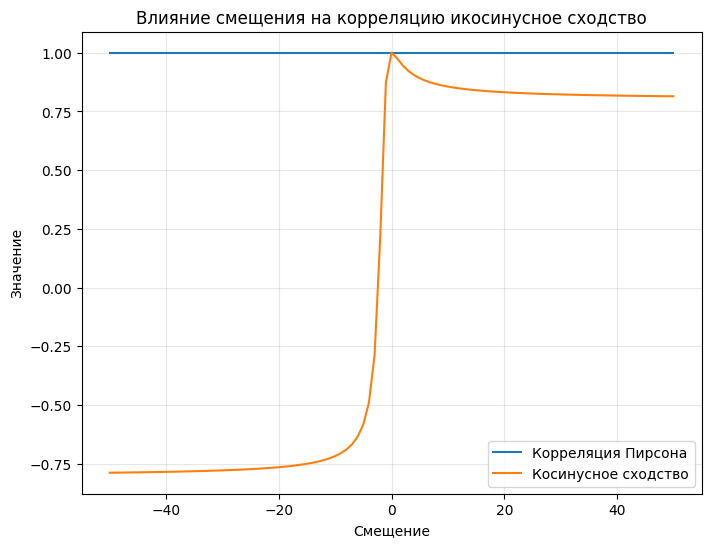
\includegraphics[width=0.8\textwidth]{./pearson_cosine.png}
    \caption{Влияние смещения на корреляцию и косинусное сходство}
    \label{fig:pearson_cosine}
\end{figure}

\section{Векторное исчисление}

\subsection*{Упражнение 5.5}

\subsubsection*{Условие}

Рассмотрим следующие функции:
\begin{align*}
f_1(x) &= sin(x_1) cos(x_2), \quad x \in \mathbb{R}^2 \\
f_2(x, y) &= x^T y, \quad x, y \in \mathbb{R}^n \\
f_3(x) &= x x^T, \quad x \in \mathbb{R}^n
\end{align*}

а. Каковы размерности матрицы \(\frac{\partial f_i}{\partial x}\)?

б. Вычислить матрицы Якоби.

\subsubsection*{Решение}

1. Функция \( f_1(x) = sin(x_1) cos(x_2), \quad x \in \mathbb{R}^2 \).

\quad

Частные производные:
\begin{align*}
\frac{\partial f_1}{\partial x_1} &= \cos(x_1)\cos(x_2) \\
\frac{\partial f_1}{\partial x_2} &= -\sin(x_1)\sin(x_2)
\end{align*}

Матрица Якоби:
\[
J_{f_1} = \frac{\partial f_1}{\partial x} = \begin{bmatrix}
\dfrac{\partial f_1}{\partial x_1} & \dfrac{\partial f_1}{\partial x_2}
\end{bmatrix} = \begin{bmatrix}
\cos(x_1)\cos(x_2) & -\sin(x_1)\sin(x_2)
\end{bmatrix}
\]

Таким образом, получили матрицу \(\frac{\partial f_1}{\partial x}\) размерностью \(1 \times 2\).

\quad

2. Функция \( f_2(x, y) = x^T y, \quad x, y \in \mathbb{R}^n \).

\quad

Координатная форма:
\[
f_2(x, y) = x^T y = \sum_{i=1}^n x_i y_i
\]

Частные производные:
\begin{align*}
\frac{\partial f_2}{\partial x_i} &= y_i \quad \text{для } i = 1, \ldots, n \\
\frac{\partial f_2}{\partial y_j} &= x_j \quad \text{для } j = 1, \ldots, n
\end{align*}

Матрица Якоби:
\[
J_{f_2} = \frac{\partial f_2}{\partial (x, y)} = \begin{bmatrix}
\dfrac{\partial f_2}{\partial x} & \dfrac{\partial f_2}{\partial y}
\end{bmatrix} = \begin{bmatrix} y^T & x^T \end{bmatrix}
\]

В развёрнутой форме:
\[
J_{f_2} = \begin{bmatrix}
y_1 & y_2 & \cdots & y_n & x_1 & x_2 & \cdots & x_n
\end{bmatrix}
\]

Таким образом, получили матрицу \(\frac{\partial f_2}{\partial x}\) размерностью \(1 \times 2n\).

\quad

3. Функция \( f_3(x) = x x^T, \quad x \in \mathbb{R}^n \).

\quad

Запись в матричном виде:
\[
f_3(x) = x x^T = \begin{bmatrix}
x_1^2 & x_1x_2 & \cdots & x_1x_n \\
x_2x_1 & x_2^2 & \cdots & x_2x_n \\
\vdots & \vdots & \ddots & \vdots \\
x_nx_1 & x_nx_2 & \cdots & x_n^2
\end{bmatrix}
\]

Рассмотрим произвольный элемент матрицы: \([f_3(x)]_{ij} = x_i x_j\).

\quad

Вычислим частные производные этого элемента по всем переменным \(x_k\): 
\begin{align*}
\frac{\partial (x_i x_j)}{\partial x_i} &= x_j, \quad \text{при } k = i, k \neq j \\
\frac{\partial (x_i x_j)}{\partial x_j} &= x_i, \quad \text{при } k = j, k \neq i \\
\frac{\partial (x_i^2)}{\partial x_i} &= 2x_i, \quad \text{при } k = i = j \\
\frac{\partial (x_i x_j)}{\partial x_k} &= 0, \quad \text{при } k \neq i, k \neq j
\end{align*}

Пусть \(x = \begin{bmatrix} x_1 \\ x_2 \end{bmatrix}\), тогда:
\[
f_3(x) = x x^T = \begin{bmatrix}
x_1^2 & x_1x_2 \\
x_1x_2 & x_2^2
\end{bmatrix}
\]

Вычислим матрицу Якоби в этом случае. Для этого сначала запишем все элементы функции в виде вектора:
\[
\text{vec}(f_3(x)) = \begin{bmatrix}
x_1^2 \\ x_1x_2 \\ x_1x_2 \\ x_2^2
\end{bmatrix}
\]

Теперь вычислим частные производные:
\begin{align*}
\frac{\partial x_1^2}{\partial x_1} &= 2x_1 &
\frac{\partial x_1^2}{\partial x_2} &= 0 \\
\frac{\partial (x_1x_2)}{\partial x_1} &= x_2 &
\frac{\partial (x_1x_2)}{\partial x_2} &= x_1 \\
\frac{\partial (x_1x_2)}{\partial x_1} &= x_2 &
\frac{\partial (x_1x_2)}{\partial x_2} &= x_1 \\
\frac{\partial x_2^2}{\partial x_1} &= 0 &
\frac{\partial x_2^2}{\partial x_2} &= 2x_2
\end{align*}

Таким образом, получаем матрицу Якоби для \(n = 2\):
\[
J_{f_3} = \begin{bmatrix}
2x_1 & 0 \\
x_2 & x_1 \\
x_2 & x_1 \\
0 & 2x_2
\end{bmatrix}
\]

В общем случае матрица Якоби имеет размерность \(n^2 \times n\). Её можно построить по блокам. Для каждого \(k = 1, \ldots, n\), столбец матрицы Якоби, соответствующий \(\frac{\partial f_3}{\partial x_k}\), представляет собой матрицу \(n \times n\):

\[
\frac{\partial f_3}{\partial x_k} = e_k x^T + x e_k^T
\]
где \(e_k\) — \(k\)-й базисный вектор.

\quad

В развернутой форме получаем следующее:
\[
\frac{\partial f_3}{\partial x_k} = \begin{bmatrix}
0 & \cdots & 0 & x_1 & 0 & \cdots & 0 \\
\vdots & \ddots & \vdots & \vdots & \vdots & \ddots & \vdots \\
0 & \cdots & 0 & x_{k-1} & 0 & \cdots & 0 \\
x_1 & \cdots & x_{k-1} & 2x_k & x_{k+1} & \cdots & x_n \\
0 & \cdots & 0 & x_{k+1} & 0 & \cdots & 0 \\
\vdots & \ddots & \vdots & \vdots & \vdots & \ddots & \vdots \\
0 & \cdots & 0 & x_n & 0 & \cdots & 0
\end{bmatrix}
\]

\subsection*{Упражнение 5.6}

\subsubsection*{Условие}

Дифференцируйте \(f\) относительно \(t\) и \(g\) относительно \(X\), где
\begin{align*}
f(t) &= \sin(\log(t^T t)), \quad t \in \mathbb{R}^D \\
g(X) &= \operatorname{tr}(AXB), \quad A \in \mathbb{R}^{D \times E}, X \in \mathbb{R}^{E \times F}, B \in \mathbb{R}^{F \times D}
\end{align*}

\subsubsection*{Решение}

1. Функция \( f(t) = \sin(\log(t^T t)), \quad t \in \mathbb{R}^D \).

\quad

Запишем её как композицию:
\[
f(t) = \sin(u(t)), \quad \text{где } u(t) = \log(v(t)), \quad \text{и } v(t) = t^T t
\]

Вычислим частные производные каждой функции:
\begin{align*}
\frac{\partial v}{\partial t} &= \frac{\partial (t^T t)}{\partial t} = 2t \\
\frac{\partial u}{\partial v} &= \frac{\partial \log(v)}{\partial v} = \frac{1}{v} = \frac{1}{t^T t} \\
\frac{\partial f}{\partial u} &= \frac{\partial \sin(u)}{\partial u} = \cos(u) = \cos(\log(t^T t))
\end{align*}

И применим правило цепочки:
\[
\frac{\partial f}{\partial t} = \frac{\partial f}{\partial u} \cdot \frac{\partial u}{\partial v} \cdot \frac{\partial v}{\partial t} = \cos(\log(t^T t)) \cdot \frac{1}{t^T t} \cdot 2t = \frac{2\cos(\log(t^T t))}{t^T}
\]

Таким образом:
\[
\frac{\partial f}{\partial t} = \frac{2\cos(\log(t^T t))}{t^T}
\]

\quad

2. Функция \( g(X) = \operatorname{tr}(AXB) \), где \( A \in \mathbb{R}^{D \times E}, X \in \mathbb{R}^{E \times F}, B \in \mathbb{R}^{F \times D} \).

\quad

Запишем след в координатной форме:
\[
\operatorname{tr}(AXB) = \sum_{i=1}^D \sum_{j=1}^E \sum_{k=1}^F A_{ij} X_{jk} B_{ki}
\]

Вычислим частную производную по элементу \( X_{mn} \):
\[
\frac{\partial g}{\partial X_{mn}} = \sum_{i=1}^D \sum_{j=1}^E \sum_{k=1}^F A_{ij} \frac{\partial X_{jk}}{\partial X_{mn}} B_{ki}
\]

Здесь мы можем воспользоваться свойством \( \frac{\partial X_{jk}}{\partial X_{mn}} = \delta_{jm} \delta_{kn} \), где \( \delta_{ij} \) — символ Кронекера, который определяется как:
\[
\delta_{ij} = \begin{cases}
1 & \text{если } i = j \\
0 & \text{если } i \neq j
\end{cases}
\]

Благодаря этому свойству двойная сумма упрощается, потому что \( \frac{\partial X_{jk}}{\partial X_{mn}} \neq 0 \) только тогда, когда \( j = m \) и \( k = n \).

Следовательно, получаем:
\[
\frac{\partial g}{\partial X_{mn}} = \sum_{i=1}^D A_{im} B_{ni}
\]

Это соответствует элементу матрицы \( B^T A^T \), но поскольку мы хотим получить \( \frac{\partial g}{\partial X} \), а не \( \frac{\partial g}{\partial X^T} \), имеем:
\[
\frac{\partial g}{\partial X} = A^T B^T
\]

\subsection*{Упражнение 5.7}

\subsubsection*{Условие}

Вычислите производные \( \frac{\partial f}{\partial x} \) следующих функций, используя правило цепочки. Укажите размеры каждой отдельной частной производной. Подробно опишите свои действия.

\quad

а.
\[
f(z) = \log(1 + z), \quad z = x^T x, \quad x \in \mathbb{R}^D
\]

\quad

б.
\[
f(z) = \sin(z), \quad z = Ax + b, \quad A \in \mathbb{R}^{E \times D}, x \in \mathbb{R}^D, b \in \mathbb{R}^E
\]
где \(\sin(\cdot)\) применяется к каждому элементу \(z\).

\subsubsection*{Решение}

а. Функция \( f(z) = \log(1 + z), \quad z = x^T x, \quad x \in \mathbb{R}^D \).

\quad

Функция представляет собой композицию:
\[
f(x) = h(g(x)), \quad \text{где } h(z) = \log(1 + z), \quad g(x) = x^T x
\]

Вычислим промежуточные частные производные.

\quad

Производная \( \frac{\partial h}{\partial z} \):
\[
\frac{\partial h}{\partial z} = \frac{\partial}{\partial z} \log(1 + z) = \frac{1}{1 + z} \quad (1 \times 1)
\]

Производная \( \frac{\partial z}{\partial x} \):
\[
z = x^T x = \sum_{i=1}^D x_i^2
\]
\[
\frac{\partial z}{\partial x_j} = \frac{\partial}{\partial x_j} \left( \sum_{i=1}^D x_i^2 \right) = 2x_j
\]
\[
\frac{\partial z}{\partial x} = 2x \quad (D \times 1)
\]

Применим правило цепочки:
\[
\frac{df}{dx} = \frac{\partial h}{\partial z} \cdot \frac{\partial z}{\partial x}
= \frac{1}{1 + z} \cdot 2x
= \frac{2x}{1 + x^T x}
\]

\quad

б. Функция \( f(z) = \sin(z), \quad z = Ax + b, \quad A \in \mathbb{R}^{E \times D}, x \in \mathbb{R}^D, b \in \mathbb{R}^E \).

\quad

Функция представляет собой композицию:
\[
f(x) = h(g(x)), \quad \text{где } h(z) = \sin(z), \quad g(x) = Ax + b
\]

Вычислим промежуточные частные производные.

\quad

Поскольку \(\sin(\cdot)\) применяется поэлементно, производная \( \frac{\partial h}{\partial z} \) представляет собой диагональную матрицу:
\[
\frac{\partial h}{\partial z} = \text{diag}(\cos(z)) = \begin{bmatrix}
\cos(z_1) & 0 & \cdots & 0 \\
0 & \cos(z_2) & \cdots & 0 \\
\vdots & \vdots & \ddots & \vdots \\
0 & 0 & \cdots & \cos(z_E)
\end{bmatrix} \quad (E \times E)
\]

Производная \( \frac{\partial z}{\partial x} \):
\[
z = Ax + b \Rightarrow \frac{\partial z}{\partial x} = A \quad (E \times D)
\]

Применим правило цепочки:
\[
\frac{df}{dx} = \frac{\partial h}{\partial z} \cdot \frac{\partial z}{\partial x}
= \text{diag}(\cos(z)) \cdot A
\]

\subsection*{Упражнение 5.8}

\subsubsection*{Условие}

Вычислите производные \( \frac{\partial f}{\partial x} \) следующих функций. Подробно опишите свои действия.

\quad

а. Используйте правило цепочки. Укажите размеры каждой отдельной частной производной.
\begin{align*}
f(z) &= \exp\left(-\frac{1}{2}z\right) \\
z &= g(y) = y^T S^{-1} y \\
y &= h(x) = x - \mu
\end{align*}
где \( x, \mu \in \mathbb{R}^D, S \in \mathbb{R}^{D \times D} \).

\quad

б.
\[
f(x) = \operatorname{tr}(xx^T + \sigma^2 I), \quad x \in \mathbb{R}^D
\]

\quad

в. Используйте правило цепочки. Укажите размеры каждой отдельной частной производной. Вам не нужно вычислять произведение частных производных явно.
\begin{align*}
f &= \tanh(z) \in \mathbb{R}^M \\
z &= Ax + b, \quad x \in \mathbb{R}^N, A \in \mathbb{R}^{M \times N}, b \in \mathbb{R}^M
\end{align*}
где \(\tanh\) применяется поэлементно к каждому компоненту \(z\).

\subsubsection*{Решение}

a. Определим структуру композиции:
\[
f(x) = f(z(g(y(h(x)))))
\]

Вычислим все частные производные.

\quad

Производная \( \frac{\partial f}{\partial z} \):
\[
\frac{\partial f}{\partial z} = \frac{\partial}{\partial z} \exp\left(-\frac{1}{2}z\right) = -\frac{1}{2} \exp\left(-\frac{1}{2}z\right) \quad (1 \times 1)
\]

Производная \( \frac{\partial z}{\partial y} \):
\[
z = y^\top S^{-1} y = \sum_{i=1}^D \sum_{j=1}^D y_i [S^{-1}]_{ij} y_j
\]
\[
\frac{\partial z}{\partial y_k} = \sum_{j=1}^D [S^{-1}]_{kj} y_j + \sum_{i=1}^D y_i [S^{-1}]_{ik} = 2 \sum_{j=1}^D [S^{-1}]_{kj} y_j
\]
\[
\frac{\partial z}{\partial y} = 2 S^{-1} y \quad (1 \times D)
\]

Производная \( \frac{\partial y}{\partial x} \):
\[
y = x - \mu \Rightarrow \frac{\partial y}{\partial x} = I_D \quad (D \times D)
\]

Применим правило цепочки:
\[
\frac{df}{dx} = \frac{\partial f}{\partial z} \cdot \frac{\partial z}{\partial y} \cdot \frac{\partial y}{\partial x}
\]
\[
\frac{df}{dx} = \left(-\frac{1}{2} \exp\left(-\frac{1}{2}z\right)\right) \cdot (2 S^{-1} y) \cdot I_D
\]
\[
\frac{df}{dx} = -\exp\left(-\frac{1}{2}y^T S^{-1} y\right) \cdot S^{-1} y
\]

Таким образом, получаем что:
\[
\frac{df}{dx} = -\exp\left(-\frac{1}{2}(x - \mu)^T S^{-1} (x - \mu)\right) \cdot S^{-1} (x - \mu)
\]

\quad

б. Функция \( f(x) = \operatorname{tr}(xx^T + \sigma^2 I), \quad x \in \mathbb{R}^D \).

\quad

Запишем внешнее произведение явно:
\[
x x^T = \begin{bmatrix}
x_1^2 & x_1 x_2 & \cdots & x_1 x_D \\
x_2 x_1 & x_2^2 & \cdots & x_2 x_D \\
\vdots & \vdots & \ddots & \vdots \\
x_D x_1 & x_D x_2 & \cdots & x_D^2
\end{bmatrix}
\]

Вычислим след:
\[
f(x) = \operatorname{tr}(x x^T + \sigma^2 I) = \operatorname{tr}(x x^T) + \operatorname{tr}(\sigma^2 I)
\]
\[
\operatorname{tr}(x x^T) = \sum_{i=1}^D x_i^2 = x^T x
\]
\[
\operatorname{tr}(\sigma^2 I) = \sigma^2 D
\]
\[
f(x) = x^T x + \sigma^2 D
\]

Вычислим производную:
\[
\frac{df}{dx} = \frac{\partial}{\partial x} (x^T x + \sigma^2 D) = 2x
\]

\quad

в. Определим структуру композиции:
\[
f(x) = \tanh(Ax + b)
\]

Вычислим частные производные.

\quad

Поскольку \(\tanh\) применяется поэлементно, производная \( \frac{\partial f}{\partial z} \) представляет собой диагональную матрицу:
\[
\frac{\partial f}{\partial z} = \text{diag}\left(1 - \tanh^2(z)\right) \quad (M \times M)
\]
\[
\frac{\partial f}{\partial z} = \begin{bmatrix}
1 - \tanh^2(z_1) & 0 & \cdots & 0 \\
0 & 1 - \tanh^2(z_2) & \cdots & 0 \\
\vdots & \vdots & \ddots & \vdots \\
0 & 0 & \cdots & 1 - \tanh^2(z_M)
\end{bmatrix}
\]

Производная \( \frac{\partial z}{\partial x} \):
\[
z = Ax + b \Rightarrow \frac{\partial z}{\partial x} = A \quad (M \times N)
\]

Применим правило цепочки:
\[
\frac{df}{dx} = \frac{\partial f}{\partial z} \cdot \frac{\partial z}{\partial x} = \text{diag}\left(1 - \tanh^2(Ax + b)\right) \cdot A
\]

\subsection*{Упражнение 5.9}

\subsubsection*{Условие}

Определим:
\begin{align*}
g(x, z, \nu) &:= \log p(x, z) - \log q(z, \nu) \\
z &:= t(\epsilon, \nu)
\end{align*}
где \(p, q, t\) — дифференцируемые функции, и \(x \in \mathbb{R}^D\), \(z \in \mathbb{R}^E\), \(\nu \in \mathbb{R}^F\), \(\epsilon \in \mathbb{R}^G\).

\quad

Требуется вычислить следующий градиент, используя правило цепочки:
\[
\frac{d}{d\nu} g(x, z, \nu)
\]

\subsubsection*{Решение}

Запишем полную производную, используя правило цепочки:
\[
\frac{dg}{d\nu} = \frac{\partial g}{\partial \nu} + \frac{\partial g}{\partial z} \cdot \frac{\partial z}{\partial \nu}
\]

Вычислим частные производные.

\quad

Производная \(\frac{\partial g}{\partial \nu}\):
\begin{align*}
\frac{\partial g}{\partial \nu} &= \frac{\partial}{\partial \nu} (\log p(x, z) - \log q(z, \nu)) \\
&= 0 - \frac{\partial}{\partial \nu} \log q(z, \nu) \\
&= -\frac{1}{q(z, \nu)} \cdot \frac{\partial q(z, \nu)}{\partial \nu} \quad (1 \times F)
\end{align*}

Производная \(\frac{\partial g}{\partial z}\):
\begin{align*}
\frac{\partial g}{\partial z} &= \frac{\partial}{\partial z} (\log p(x, z) - \log q(z, \nu)) \\
&= \frac{1}{p(x, z)} \cdot \frac{\partial p(x, z)}{\partial z} - \frac{1}{q(z, \nu)} \cdot \frac{\partial q(z, \nu)}{\partial z} \quad (1 \times E)
\end{align*}

Производная \(\frac{\partial z}{\partial \nu}\):
\[
\frac{\partial z}{\partial \nu} = \frac{\partial t(\epsilon, \nu)}{\partial \nu} \quad (E \times F)
\]

Подставлим в формулу полной производной:
\[
\frac{dg}{d\nu} = -\frac{1}{q(z, \nu)} \cdot \frac{\partial q(z, \nu)}{\partial \nu} + (\frac{1}{p(x, z)} \cdot \frac{\partial p(x, z)}{\partial z} - \frac{1}{q(z, \nu)} \cdot \frac{\partial q(z, \nu)}{\partial z}) \cdot \frac{\partial t(\epsilon, \nu)}{\partial \nu}
\]

\end{document}